\documentclass{article}
\usepackage[utf8]{inputenc}
\usepackage[a4paper, total={6in, 8in}]{geometry}
\usepackage{braket}
\usepackage{xcolor}
\usepackage{amsmath}
\usepackage{amsfonts}
\usepackage{graphicx}
% \usepackage{biblatex} %Imports biblatex package
\usepackage{float}
\usepackage{media9}

\usepackage[
backend=biber,
style=alphabetic,
sorting=ynt
]{biblatex}

\addbibresource{sample.bib} %Import the bibliography file

\newcommand{\commentt}[1]{\textcolor{blue}{ \textbf{[COMMENT]} #1}}
\newcommand{\ctt}[1]{\commentt{#1}}
\newcommand{\prb}[1]{ \mathbf{Pr} \left[ {#1} \right]}
\newcommand{\onotation}[1]{\(\mathcal{O} \left( {#1}  \right) \)}
\newcommand{\ona}[1]{\onotation{#1}}

\title{Introduction to Quantum Computing}
\author{David Ponarovsky}
\date{August 2021}

\begin{document}
\graphicspath{ {./images/} }
\maketitle

\part{ Problems }

\paragraph{Ex1 - Quantum Communication Complexity of Disjointness.}
Consider the following communication
problem. As inputs Alice gets an \(x\) and Bob get a \(y\), where \(x, y \in \{0, 1\}^n \), and by exchanging information they what to determine if there is an index \(k\) with \(x_k = y_k = 1 \) or not. 
In other words, if \(x\) encodes the
set \(A = \{k | x_k = 1\} \), and \(y\) encodes \(B = \{k | y_k = 1\}\), then Alice and Bob want to determine whether \( A \cap B \) is empty or not.

The classical randomized communication complexity of this problem is \ona{n}.
Assuming Alice and Bob can exchange quantum messages, show how Alice and bob can solve the task
correctly with probability greater than \(2/3\) by exchanging at most \ona{n\log n } qubits.

\paragraph{Solution} Let \( x^{(j)} \) be the \(j\)-th \(\sqrt{n}\)-block of \(x\), e.g \(x^{(j)} = x_{j\sqrt{n}},x_{j\sqrt{n}+1}...,x_{(j+1)(\sqrt{n})-1}  \). And denote by \( \ket{\psi_x} \in \mathcal{H}_{2}^{\bigotimes \sqrt{n}} \bigotimes \mathcal{H}_{\sqrt{n}} \) the uniform superposition state over the \( x^{(j)}\)-'s "tensored" with \(\sqrt{n}\)-qudit (which will correspond to the block number).  \[ \ket{\psi_x} = \frac{1}{n^\frac{1}{4}}\sum_{j}^{\sqrt{n}}\ket{x^{(j)}}\ket{j} \] Note that \( \ket{\psi_x} \) require only \( \sqrt{n} + \log(\sqrt{n}) \) qubits. Suppose Alice and Bob can generate the states \( \ket{\psi_x}, \ket{\psi_y} \) in polynomial time, then Bob sends he's share to Alice. We know that there is a classical circuit with logarithmic depth in \( \sqrt{n} \) that act over the pure states \( \ket{x^{(j)}}\ket{j} , \ket{y^{(k)}}\ket{k} \) and decides whether \[ \left( j =  k \right) \ \mathbf{AND}  \ \left( x^{(j)} \ \mathbf{bitwise-OR} \  y^{(k)} \right)   \]

Denote it by \( C \) and it's quantum version of that circuit by \( U \), which is operator in Hilbert state at dimension: \[ \mathcal{O} \left( \left( \dim \left( \mathcal{H}_{2}^{\bigotimes \sqrt{n}} \bigotimes \mathcal{H}_{\sqrt{n}} \right) \right) ^2 o(1) \right) = \mathcal{O} \left( 2^{2\sqrt{n}}  \right)  \]
Suppose that \( A \cap B \neq \emptyset \) then, the support of \( \ket{\psi_x} \otimes \ket{\psi_y} \) contain a state \( \ket{\phi} \) which satisfies \(C\), and therefore  after performing \ona{ 2^{ \sqrt{n}}} Grover iterations, measuring the qubits "type" will collapse (\textbf{w.h.p}) into \( \ket{\phi} \). In another hand, if \( A \cap B = \emptyset \) then no matter what will be the result of the measurement, Alice could could verify it by applying the classical circuit. 
\paragraph{}Summarize the above yields the following protocol,
\begin{enumerate}
    \item Bob create \( \ket{\psi_x} \) and sent it to Alice.
    \item Alice uses Grover search and \(U\) to amplify the probability to measure a state \( \ket{\phi} \in Support \left(   \ket{\psi_x} \otimes \ket{\psi_y}  \right) \) that satisfies \(C\).
    \item denote by \( \tilde{\phi} \) the result (a bit string / pure state) that Alice measured, Alice compute \(C\left(\tilde{\phi}\right) \) and returns the result. 
\end{enumerate}
The corrections, emits directly from Grover corrections and the construction above, the probability to measure an instruction between \(A\) and \(B\) is grater than \( \frac{2}{3} \) in case there is exist such, due to Grover. In the case the instruction is empty Alice will returns false at probability equal 1 (as explained above). The communication cost is exactly  \( \sqrt{n} + \log(\sqrt{n}) \) qubits.  
\paragraph{Ex2 - Quantum Fingerprinting }
\begin{enumerate}
    \item (P1) Consider the following “Swap Test”: Given two states \( \ket{\phi_x}\), \( \ket{\phi_y}\) in some Hilbert space \( \mathcal{H}\),
show that the probability of measuring a \(0\) outcome in the following quantum circuit is \( \mathbf{Pr} [ \mathbf{ \ TEST} = \ket{0} \   ]  =  \frac{1}{2} \left(1 + \norm{\braket{\phi_x| \phi_y}}^2 \right) \) .

\textbf{Solution.} Let's calculate the state before the measurement: 
\[ \begin{split}
    H \ \mathbf{SWAP} \ H \ket{\psi_x \psi_y 0} & = \mathbf{SWAP} \ H \frac{1}{\sqrt{2}}\left( \ket{\psi_x \psi_y 0} + \ket{\psi_x \psi_y 1}\right) \\
    & = H \frac{1}{\sqrt{2}}\left( \ket{\psi_x \psi_y 0} + \ket{\psi_y \psi_x 1}\right)\\ &= \frac{1}{2}\left(  \ket{\psi_x \psi_y 0} + \ket{\psi_y \psi_x 0}  + \ket{\psi_x \psi_y 1} - \ket{\psi_y \psi_x 1}\right)
\end{split}  \]
Thus, the probability to measure \( 0 \) equal \( \frac{1}{4}\left(  \braket{ \psi_x \psi_y | \psi_x \psi_y } + \braket{\psi_y \psi_x | \psi_y \psi_x } + 2 \braket{\psi_y \psi_x|\psi_x \psi_y} \right) \)
by the fact that inner product is symmetric to conjugation, we get: 
\[ \braket{\psi_y \psi_x|\psi_x \psi_y} = \braket{\psi_y | \psi_x}\braket{\psi_x | \psi_y} = \braket{\psi_x | \psi_y}\braket{\psi_x | \psi_y} = \braket{\psi_x | \psi_y}^2 \] Therefore the probability is \( \frac{1}{4}\left(2 + 2 \braket{\psi_x | \psi_y}^2 \right) =  \frac{1}{2}\left(1 +  \braket{\psi_x | \psi_y}^2 \right)   \)  

\item  (P2) Let \( \mathcal{H}\) be a Hilbert space of dimension \(m\). Show that one find exponentially many “almost orthogonal” states in \( \mathcal{H}\). Namely, for any \( \varepsilon > 0 \)   there is a constant \(c = c(\varepsilon) > 0 \), and states \( \ket{\phi_k} \ k = 1,...,2^{cm} \), such that for all \(k \neq j \) we have \( \norm{\braket{\phi_k| \phi_j}}^2 \le \varepsilon \) 


\textbf{Solution.} As the hint implies let's look on \( 2^{cm} \) random states \( \{ \ket{\psi_k} \}_{0}^{2^{cm}}\), such that \( \ket{\psi_k} = \frac{1}{\sqrt{m}}\sum_{i}^{m}{X_{ik}\ket{i}} \). Where \( X_{ik} \) distributed uniformly over \(X_{ik} \sim  \{ -1 , 1 \} \). We want to show that \[
\mathbf{Pr} \left[ \exists k \neq j ; \braket{\psi_k| \psi_j} \ge \varepsilon \right] < 1 \] When the probability is over the \( X_{ik} \)-'s. If the inequality holds, then It's mean that there is at least one assignment of the \( m2^{cm} \) \(X_{ik}\)-'s variable such that the \( 2^{cm} \) states combine an "almost orthogonal" base. Let's bound that probability, first let's move to bounded random variables ( in \( [0,1] \) ) with positive expectation. ( required conditions for \textbf{Hoeffding}'s inequality ).  

\[ 
\begin{split}
\mathbf{Pr} \left[ \exists k \neq j ; \braket{\psi_k| \psi_j} \ge \varepsilon \right]  &= 
\mathbf{Pr} \left[ \exists k \neq j ; \frac{1}{2} \left( 1 + \braket{\psi_k| \psi_j} \right) \ge \frac{1}{2} \left( 1 + \varepsilon \right) \right]  \\
& \le \sum_{k\neq j } {\mathbf{Pr} \left[ \frac{1}{2} \left( 1 + \braket{\psi_k| \psi_j} \right) \ge \frac{1}{2} \left( 1 + \varepsilon \right) \right] } \\ 
& \le 2^{2cm} \mathbf{Pr} \left[ \frac{1}{2} \left( 1 + \braket{\psi_k| \psi_j} \right) \ge \frac{1}{2} \left( 1 + \varepsilon \right) \right] \\ 
& \le  2^{2cm}  \mathbf{Pr} \left[  \frac{1}{m}\sum_{i}^{m} \frac{1}{2} \left( 1 + X_{ik}X_{ij} \right) \ge \frac{1}{2} \left( 1 + \varepsilon \right) \right] \\
& \le 2^{2cm}e^{-\frac{m}{2}\varepsilon^2} < 1 \Rightarrow c(\varepsilon) < \frac{1}{2m} \log_{2} \left( e^{\frac{m}{2}\varepsilon^2} \right) = \frac{1}{2} \log_{2} \left( e^{\frac{1}{2}\varepsilon^2} \right)
\end{split}
\]
Where the second transition is due to the union bound and the last is due to Hoeffding. Notice that, \(c\) doesn't deepened over \(m\) which implies that the bound is far from been tight.    
\end{enumerate}
Now consider the following simultaneous communication problem. Alice and Bob do not share any entanglement or any common randomness, and cannot communicate directly with each other. As
inputs, \(x\) is given to Alice, and \(y\) is given to Bob, where \(x, y \in \{0, 1\}^n \). Based on their inputs Alice and Bob can each send a single message to a referee \(R\) that has to decide whether \(x = y\) or not.

\begin{enumerate}
    \item Give a quantum protocol where Alice and Bob each send to \(R\) a quantum state on \ona{ \log n}  qubits and the error probability of R is at most \( 1/100\) 
    
    
    \textbf{Solution.} Let \(m^\prime\) be an integer such that \( 2^{c(\varepsilon)m^\prime} = n \Rightarrow m^\prime = \frac{\log n}{c(\varepsilon)}\), by (a) there exists a \(2^n\) states \( \{ \ket{\psi_k} \} \) which are "almost orthogonal" ( relative to \(\varepsilon\) ). Alice and Bob send \(t\) copies of \( \ket{\psi_x} \) and \( \ket{\psi_y} \) to \(R\) . Then \(R\) execute the \textbf{SWAP TEST} \(t\) times, then if the distance of the arithmetic mean from \( \frac{1}{2} \) is lower then \(\varepsilon \) it (\(R\)) return yes, otherwise it return no.
    
    if \( x \neq y\) then the probability to get 0 in a single test is at least \( \frac{1}{2} \left( 1+ \varepsilon^2\right) \). Thus, by Hoeffding, we get again that \[ \mathbf{Pr} \left[ \frac{1}{t}\sum_{0}^{t}{ \mathbf{TEST_i} } \ge \varepsilon \right] \le e^{-2t\left( \varepsilon - \frac{\varepsilon^2}{2} \right)} \] Which yields the desirable soundness for \( \varepsilon = \frac{1}{4} \) and \( t = 100 \).   
    On the other hand, if \(x = y\) than \(R\) executes the \textbf{SWAP TEST} over the same sates, so the probability to get 0 is \(\frac{1}{2}\left(1 +  \braket{\psi_x | \psi_x}^2 \right) = 1\). Therefore \(R\) will return the right answer. 
    
    The communication complexity is exactly \( \frac{2t}{c(\varepsilon)}\log n\) qubits.
\item What is the complexity of the quantum circuits that are needed for Alice, Bob and referee \(R\), to implement the protocol suggested in (a)? Explain/Prove why.

\textbf{Solution.} An algorithm that for a given string \( x \in \{0,1\}^n \) compute the matched reduced state over \(m\) qubits in polynomial time and sub exponential memory is presented in the next question.

I am sure that it impossible to implement the protocol with only polynomial space cost.        

\item (Optional) Describe an efficient (polynomial time complexity) protocol with \ona{\log n} qubits messages from Alice and Bob to \(R\). Hint: You can use a simple classical code (not necessarily binary)
with \(2^n\) codewords, that have a good distance (and a reasonable, even if not optimal, rate). Note: There is a classical randomized algorithm where Alice and Bob each send to \(R\) a message of size \ona{\sqrt{n}}  and \(R\)’s error probability is at most \(1/100\) (This is known to be optimal).


\textbf{Solution.} polynomial time, \( \log^2(n) \) communication and \textbf{sub-exponential space}.  

\textit{First solution}, observe that there is a naive solution which require exponential space, Alice, Bob and R, holds for each \( \ket{x} \in \{0,1\}^n \) a circuit \( C_x \) which embeds the state in the \(m\)-qubits Hilbert space according to preselected base.

The description of \(C_x\) is lay below (Figure 2), and it's using \ona{ 2^{m} } \( = \) \ona{n} ancilas, by the recursive relation for the binary search gate (\(b_m\)) in Figure 1, \( T(m)= m-1 + 2T(m-1)\). The recursive relation for the depth is \( D(n)=n + D(n-1) \). Hence, the depth of \(C_x\) is \ona{n}. As said above, Alice, Bob and R, holds for every  \( \ket{x} \in \{0,1\}^n \) a circuit \(C_x\) so the total space complexity is \ona{2^n \cdot n}. 

So Alice and Bob should first perform a classic binary search at \ona{\log(2^n)} time to find the circuits \(C_x , C_y\) according to their strings \(x,y\), then each of them reduces his number \(x\) (or \( y \)) into a state \( \ket{\psi} \in \mathcal{H}_{2^m} \) and send it to \(R\). Finally \(R\) perform the \textbf{SWAP} Test and deiced whether or not \(x = y\). Therefore the total running time that required to perform that protocol is \(
    \mathcal{O}\left(log(2^n) + Depth(C_x) + \mathbf{SWAP}\right) = \mathcal{O}\left(n\right)      
\).
\begin{figure}[H]
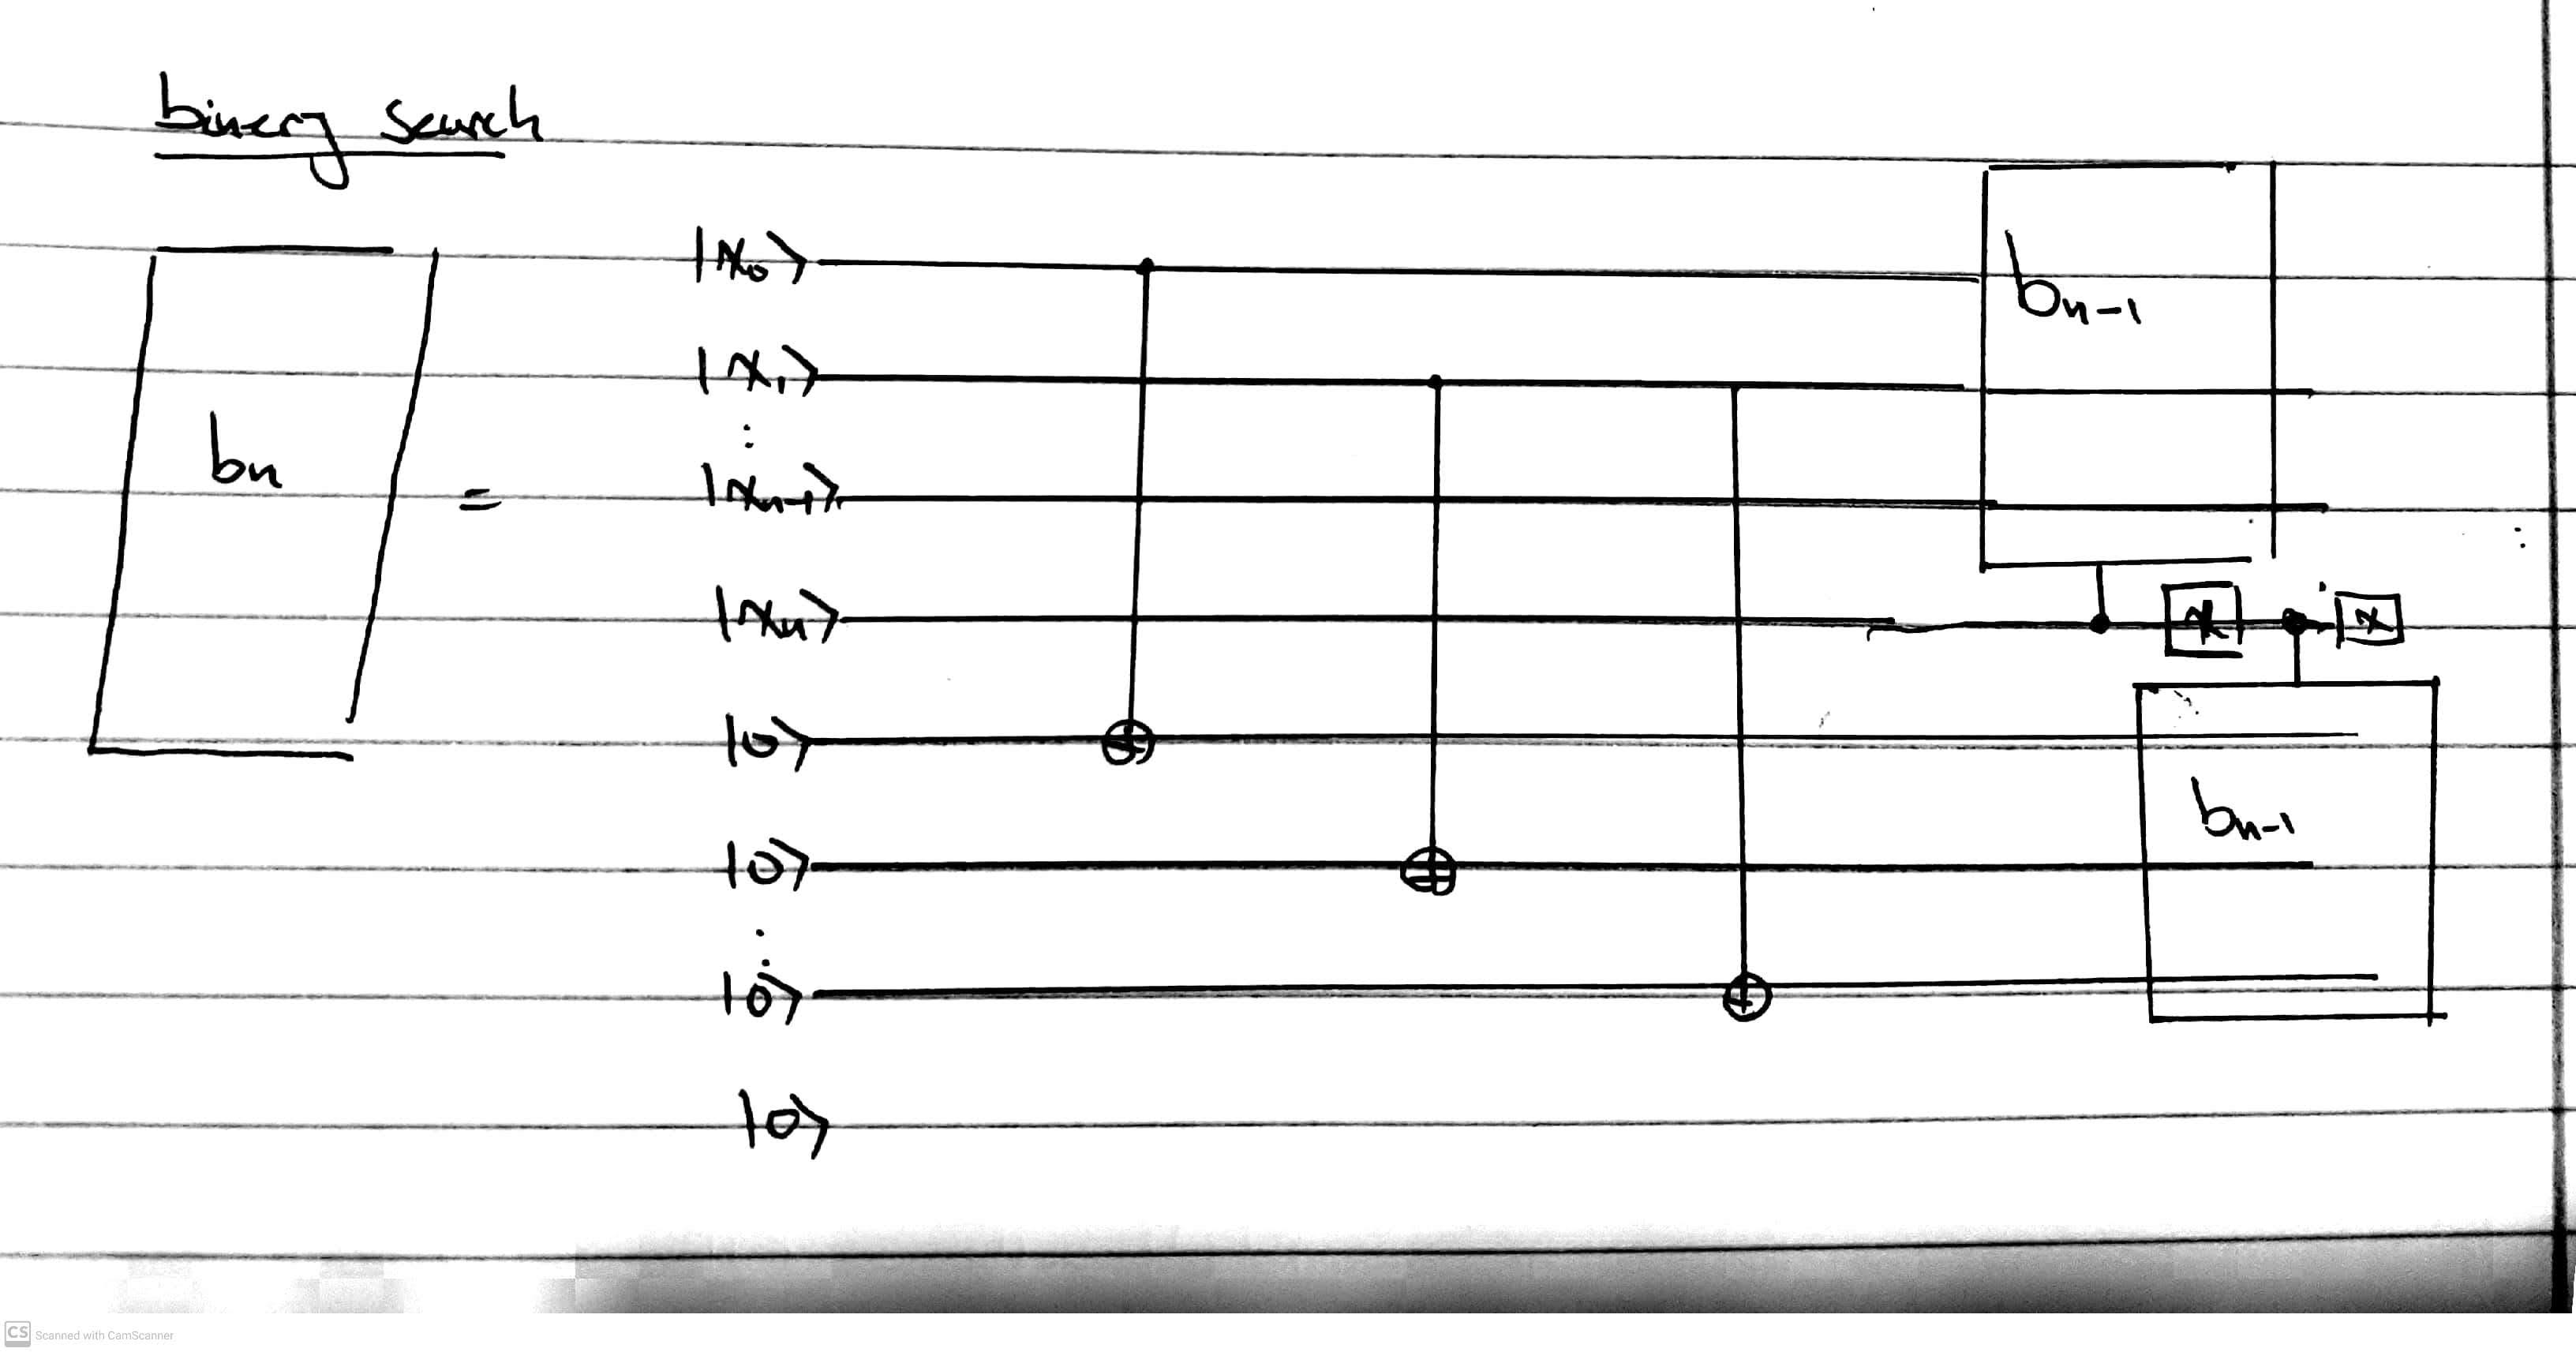
\includegraphics[scale=0.13]{binarysearch}
\caption{Binary search gate, \(b_1\) plays the role of "terminate condition" and will turn a unique qubit such that \(b_m\ket{i}\ket{0}^{\otimes O(m)} \mapsto \ket{i}\ket{junk}\ket{0}^{i}\ket{1}\ket{0}^{m-i}\). }
    \label{fig:simulation_cases}
\end{figure}


\begin{figure}[H]
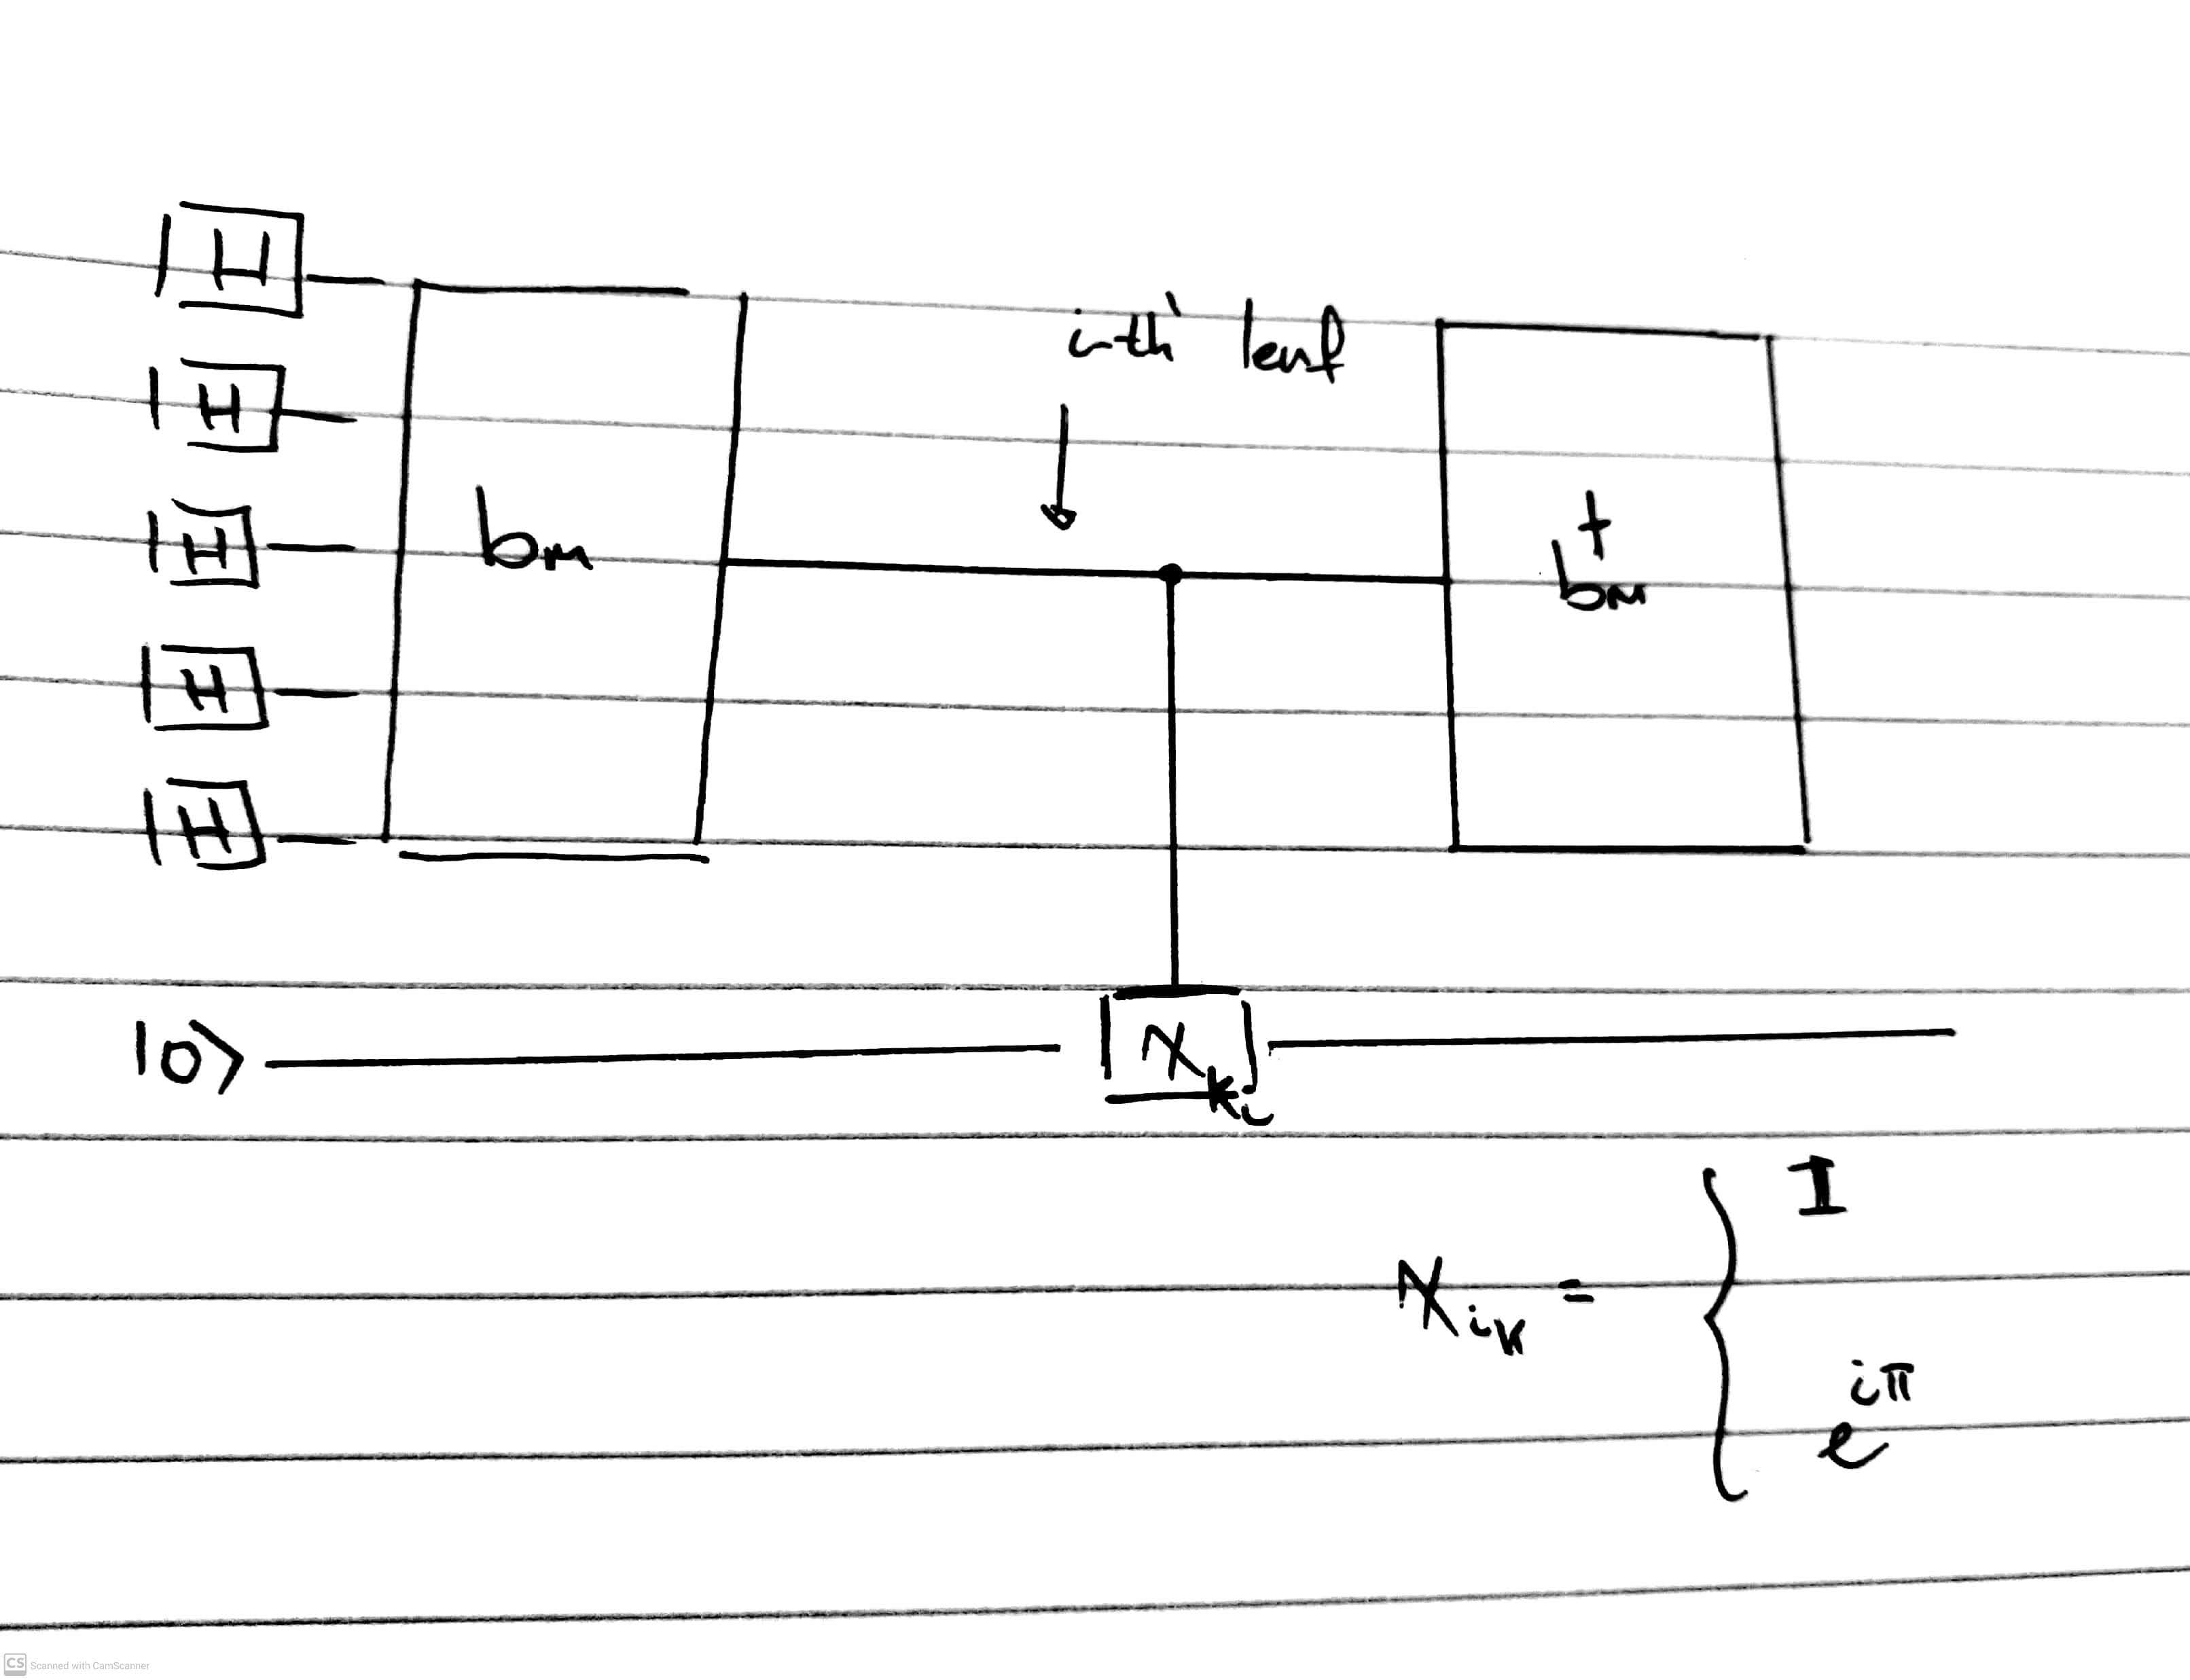
\includegraphics[scale=0.13]{binarysearch_2}
\caption{The circuit \( C_x \) which transforms the state \(\ket{0}^{\otimes m}\) into \(\frac{1}{\sqrt{m}}\sum_{i}^{m}{X_{ik}\ket{i}}\). First transform the state into the uniform super position, and then applying a "kick phase" over each ket \( \ket{i} \). the \(b_m\) perform the transformation \(b_m \frac{1}{\sqrt{m}}\sum_{i}^{m}{\ket{i} \ket{0}^{\otimes m} } \mapsto \frac{1}{\sqrt{m}}\sum_{i}^{m}{\ket{i} \ket{0}^{i }}\ket{1}\ket{0}^{m - i }  \)  which enables to multiplies only the \(\ket{i}\)-ket by the \(X_{ki}\) phase. }
    \label{fig:simulation_cases}
\end{figure}

\textit{Second solution}, with \( \log^2(n) \) communication cost and \textbf{sub-exponential space}. Alice and Bob will divide their numbers into \(\log(n)\) slices, \(x=x_1x_2...x_{\log(n)}\) ( \(y=y_1y_2...y_{\log(n)}\) ) each at length \( \frac{n}{\log(n)} \) and repeat over the protocol above \(\log(n)\) times, in each time Alice and Bob ask R if \(x_i = y_i\). Hence they will be required to hold only \( 2^{\frac{n}{\log(n)}} = 2^n/n \) circuits, which is equal to \ona{(1+\delta)^n} for every \(\delta > 0\).

And that implies a sub-exponential memory complexity, \ona{ n\log(n)} time, and \ona{\log^2(n)} communication cost.   

\end{enumerate}


\part{REVIEW} 

\section*{Constructing quantum codes from any classical code and
their embedding in ground space of local Hamiltonians. Ramis Movassagh, Yingkai Ouyang [QIP21] }
\paragraph{Introduction and results} Dealing also with phase flip errors enhances the hardness (difficulty) of finding new good error correction codes. Even there are a known wide range of classical codes with good parameters ( and with low density parity check matrix ), the generalization of their quantum version is still not a trivial task, and the question whether is there exists a quantum \textbf{LDPC} code is still open. To understand the difficulty, let us look at one of the most familiar method to construct an quantum correction code from classical. The \textbf{CSS} family, encounter each of the error types in turn. The encoding is basically goes as follow: take your state, encodes it by \( \mathcal{C}_1 \) code,  "rotates" it, and encodes it by \( \mathcal{C}_2 \). When in the rotated base, the phasefilp operation is equivalence to bitflip rotation, therefore an error can be corrected by a classical scheme. 
The problem is that the \textbf{CSS} construction requires that  \( \mathcal{C}_{2}^{\perp} \subset \mathcal{C}_{1}\). 

In the first part of the paper \textbf{Movassagh} and \textbf{Ouyang} propose a different approach to quantumize a classical code which can be applied over a bigger family of classical codes. In a nutshell, unlike the \textbf{CSS} in their construction, each logic qubit is encoded as a specific superposition combination over the codewords (equation 1) and the wights are chosen in such way that the state is "apathetic" to phase errors (till the distance). They have formulated a LP which for a given code, finds those weights, and showed that if the program is not feasible,still one could find a good approximation.  

In the second part of the article, they coin the term subspace LDPC code by  introduce a code which is a subspace of the span local Hamiltonians ground states; called also ground space. The fact that the Hamiltonian is 2-local ensures the low density of the check matrix. and the teachings from the first part have used to prove that the code has linear distance. 

\commentt{They also proved that the fraction of the code relative to the ground space aims to constant as \(n \rightarrow \infty \) which from computational point of view implies that the code is efficient (consumes bounded overhead cost).} 

\paragraph{Part I}

Denote by \( C \) classical code of distance \(d_X\). They present a logic qubit as a mixed state of codewords, for example, encode binary field might look as      

\begin{align}
    \ket{0_L} &= \sum_{{\bf c} \in C_0}  \alpha^{(0)}_{\bf c}\ket{{\bf c}} , \quad 
    \ket{1_L} = \sum_{{\bf c} \in C_1}  \alpha^{(1)}_{\bf c}\ket{{\bf c}} , \label{form1}
\end{align}
where \(C_1 , C_2\) are disjoint subspace of \(C\). let \( P \in \{ X^eZ^f \} \) such that \( e \le d_X \) and \( f \le d_Z \) be an error operator, if we can ensure that \( \braket{0_L|P|1_L} = 0 \) and \( \braket{0_L|P|0_L} = \braket{1_L|P|1_L} \) (non-deformation and orthogonality conditions) than we can tolerate the error weight. Intuitively the first condition can be thought as an ensuring that \( P \) couldn't transfer probability weights between different logical quibit, while the second condition ensures that the logical states loose (or gain) the same amount of weights after the error occur. 

\textbf{Note} That first condition \( \braket{0_L|P|1_L} = 0 \) stems directly from the assumption that \( e \le d_X \). The second condition requires the most of the work.   

\paragraph{}
 
Denote by Alg1 their proposed algorithm. The algorithm outputs the logical states:
\begin{align}
    \ket{j_L} &= \sum_{{\bf c} \in C_j}  \alpha^{(j)}_{\bf c}\ket{\bf c} , \quad 
    j\in\{0,1,\dots,M-1\} , \label{formM}
\end{align}
where \(M\le q^{c\:n}\) with \(0<c<1\) resulting in quantum codes with constant rate. They prove the following theorem:

\paragraph{Theorem.}
Take a classical code \(C\) of length \(n\) on a \(q\)-ary alphabet with 
the distance of $d_X$. Let $V_{q}(r)$ be the Hamming ball of radius \(r\). If  \(|C|\ge 2V_{q}(d_Z-1)\), then Alg1 derives  \(2 \le M\le q^{c\:n}\),quantum logical states (with \(0<c<1\))  with a bit-flip and phase-flip  distances of \(d_X\) and \(d_Z\) respectively. The overall  distance is \(\min(d_X,d_Z)\).

\paragraph{}
Note, that in case we are interested in a distance which linear in \(n\) then  \(V_{q}(d_Z)\) grow exponential \( \sim \mathcal{O}(q^n) \), but for many codes \( |C| \) is also exponential in \( n\). Therefore, it seems that this approach will cover a much wider range of codes than the \textbf{CSS}. The authors have demonstrated in the paper explicit examples for quatinze familiar codes schemes.   
\paragraph{Explicit review of binary logic qubits.} let \(x\) be a vector in \(  \mathbb{R}^m\), denote by \(x^{\pm}\) the vector such that \(x^{\pm}_{j} = \max (0, \pm x_j )\). Note that for every \(j\in [m]\) at least one of \(x^{+}_j, x^{-}_j\) is zero, and therefore \( x^{+}_jx^{-}_j = \max (0, x_j )\max (0, - x_j ) = 0 \Rightarrow \mathbf{x^{+}}\mathbf{x^{-}} = 0 \). So enforcing the logical qubits \( \ket{0_L}, \ket{1_L} \) to have an amplitudes of that form, ensures the orthogonal relation \( \braket{0_L | 1_L } = 0\).

\begin{eqnarray}
|0_{L}\rangle & = & \frac{1}{\sqrt{x}}\left(\sqrt{x_{1}^{+}}|{\bf c}_{1}\rangle+\cdots+\sqrt{x_{m}^{+}}|{\bf c}_{m}\rangle\right)\;,\label{eq:Logical0}\\
|1_{L}\rangle & = & \frac{1}{\sqrt{x}}\left(\sqrt{x_{1}^{-}}|{\bf c}_{1}\rangle+\cdots+\sqrt{x_{m}^{-}}|{\bf c}_{m}\rangle\right)\;.\label{eq:Logical1}
\end{eqnarray}

Therefore, by the fact \(e < d_X \), the orthogonality condition \( \braket{0_L|P|1_L} = 0 \) holds.  it has been left to find such \(x\)'s which will satisfy the non-deformation condition \( \braket{0_L|P|0_L} = \braket{1_L|P|1_L} \). writing those requirement as a linear program yields the constraint \( \braket{c|P|c} = 0 \) for each \( c \in \mathcal{C} \) and an error \(P\) at the form \( P = Z^f  \) such that \( f < d_Z \).     



For any classical string \(\bf c =(c_{1},\dots,c_{n})^T\in{C}\) with \(c_i = 0,1,\dots,q-1\), the quantum state is \(|{\bf c} \rangle=|c_1,c_2,\dots,c_n\rangle\), and 
when \(P = Z^{z_1}\otimes \dots \otimes Z^{z_n}\), we have
\begin{align}
    \braket{\bf c|P|\bf c} 
    =& \prod_{j=1}^n \braket{c_j|Z^{z_j}|c_j} = \prod_{j=1}^n \braket{c_j|\sum_{k\in\Sigma_c} (\omega^k)^{z_j} |k}\braket{k|c_j}=\prod_{j=1}^n \omega^{z_j c_j} =\omega^{{\bf z}^{T}{\bf c}}
    \\
    =&\cos\left(\frac{2\pi\,{\bf z}^{T}{\bf c}}{q}\right)+i\sin\left(\frac{2\pi\,{\bf z}^{T}{\bf c}}{q}\right).\label{eq:cosine-sine}
\end{align} 

And the matrix will take the form of  

\begin{equation}
A'=\sum_{w=1}^{d_Z-1}
\sum_{\wt({\bf z}) = w}
\sum_{{\bf c}\in{C}}
\left[
\cos\left(\frac{2\pi\,{\bf z}^{T}{\bf c}}{q}\right)|{\bf z},0\rangle\langle{x_c}|+
\sin\left(\frac{2\pi\,{\bf z}^{T}{\bf c}}{q}\right)|{\bf z},1\rangle\langle{x_c}|
\right].
 \label{eq:Aprime}
\end{equation} 

thus, the solution for the LP defined by \( \vec{1}\bf x = 0 \) and  \( A^\prime  \bf x = 0 \) defines the corresponding \(0,1\) code words. Furthermore, by the fact that \( \mathbf{z}^T\mathbf{c}\) are integers, the entries of the matrix are elements of a finite-sized set given by, \( \{\cos(\frac{2\pi k}{q}) , \sin(\frac{2\pi k}{q}) : k = 0, . . . , q - 1 \}\) (The feasibility proof relies on that fact).   

Again, note that the protocol has uses the entire classical code to represent only a single logical qubit. The rest of the part deals with generalizing the protocol to allow encoding a qudit, and proving that, except the rare case that the set of linear constraints have rows that are all non-zero and are of the same sign, their algorithm finds a feasible solution . 


\paragraph{Part II}

Let us consider a spin chain of length
$n$ with open boundary conditions and the local Hilbert space dimension of $2s+1$, where $s\ge1$
is a positive integer. We take a representation in which $|j\rangle$
denotes the $s_{z}=j$ state of a spin-$s$ particle:
\[
\hat{S}_{z}|j\rangle=j\;|j\rangle,\qquad j\in\Sigma\quad.
\]

The local Hamiltonian whose ground space will be shown to contain a nontrivial quantum
error correcting code is
\begin{equation}
H_{n}=H_{n}^{J}+H_{n}^{s}\label{eq:H}
\end{equation}
where \(H_{n}^{J}=J\sum_{k=1}^{n}\left(|0\rangle\langle0|\right)_{k}\).
Recall that the Hamiltonian \(H_{n}^{s}\), is defined by
\begin{equation}
H_{n}^{s}=\sum_{k=1}^{n-1}\left\{ \sum_{m=-s}^{s}P_{k,k+1}^{m}+\sum_{m=1}^{s}Q_{k,k+1}^{m}\right\} \;,\label{eq:Hn_s-2}
\end{equation}
and the local terms are projectors acting on two neighboring spins \(k,k+1\) defined by 
\begin{equation}
P^{m}=|0\leftrightarrow m\rangle\langle0\leftrightarrow m|\;,\qquad Q^{m}=|00\leftrightarrow\pm m\rangle\langle00\leftrightarrow\pm m|;\label{eq:hs_Proj}
\end{equation}

Those local projections match to local actions, \(P^m\) could be thought as spin exchanging \( m0 \leftrightarrow 0m \) and \(Q^m\) could be thought as local creation or annihilation \(00 \leftrightarrow m,-m\). They also define an equivalence class, all the states that can be reached from state \( \mathbf{t} \) by applies only \( P^m, Q^m\) operators are composite a class. The delegate of the class \( \ket{c_{x_1 x_2 x_3 .. x_k}} \) is the string such all it's zeros  adjacent to right, i.e \(  \ket{c_{x_1 x_2 x_3 .. x_k}} = \ket{x_1}\ket{x_2}\ket{x_3}..\ket{x_k}\ket{0}\ket{0}...\ket{0} \). All the definitions above have enabled them to formulate the following lemma over the specific type of ground states:      

\paragraph{Lemma} The uniform superposition of all strings in an equivalence
class (i.e., equivalent to the irreducible string 
 is a (frustration free) zero energy ground state of $H^s_n$.

\paragraph{Short explanation.} Frustration free property means that the ground state of the Hamiltonian is also the ground state for each local Hamiltonian \(H_i\). If a ground state $\psi$ vanishes
on each local projector \(P^m , Q^m\), then for any $m\in[s]$ it must obey $\langle\psi|0m\rangle=\langle\psi|m0\rangle$,
$\langle\psi|0(-m)\rangle=\langle\psi|(-m)0\rangle$ and $\langle\psi|00\rangle=\langle\psi|m(-m)\rangle$.
It follows that $\psi$ has the same amplitude on a pair of equivalent
strings ${\bf s}\sim{\bf t}$, which means $\langle\psi|{\bf s}\rangle=\langle\psi|{\bf t}\rangle$.
It follows that the ground subspace of $H_{n}^{s}$ is frustration
free and is spanned by the pairwise orthogonal states
\begin{equation}
|c_{{\bf x_{k}}}\rangle\propto\sum_{{\bf s}\sim c_{{\bf x_{k}}}}|{\bf s}\rangle\label{eq:AllGroundStates}
\end{equation}
where to simplify the notation, denote ${\bf x_{k}}=(x_{1},\dots,x_{k})$.
Clearly each distinct ${\bf x_{k}}$ results in a distinct ground
state $|c_{{\bf x_{k}}}\rangle$. 


\paragraph{The code.} In the case that \(k = n\) the equivalent class  \(\mathbf{c_{x_{k}}} \) contains exactly single state, the product \( \ket{x_0 x_1 x_2 .... x_n} \). And the collection of those pure states can be thought as a classical code which its spans reside in the ground space. Denote it by \(C\) . Finally, they have show that \( C \) satisfy the requirements of their first Theorem, that is, \( |C| \ge 2V_q \left(d_Z -1 \right) \) and that yields a linear code which is subset of the ground space of the local Hamiltonian. the total distance \( \min \left( d_Z, d_X \right) \) is linear at \(n\). Last important note, they also show that the size of code fraction from the ground space where \(n\rightarrow\infty\) aims to \( \frac{|C|}{ |ground\ H |} \rightarrow \sqrt{\frac{s-1}{s}} \). The constant ratio could be thought as "affordable" overhead cost.


\end{document}